\documentclass[tikz,margin=2mm]{standalone}
\pagestyle{empty}

\usepackage{amsmath}
\usepackage{bm}
\usetikzlibrary{positioning,calc, arrows,shapes}

\begin{document}
	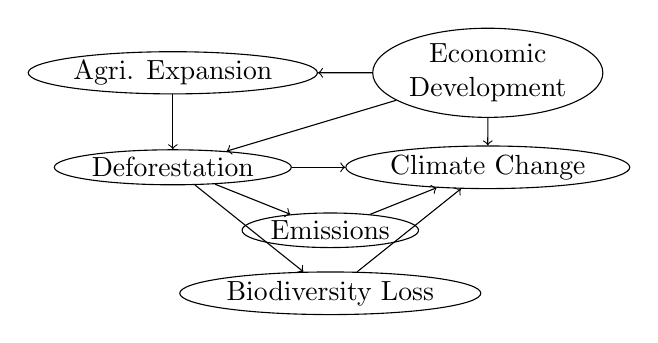
\begin{tikzpicture}
		\begin{scope}[scale=0.8]
		\tikzstyle{every node}=[draw, ellipse, align=center, inner sep=1pt]
				\node (D) at (0, 0) {Deforestation};
				\node (CC) at (5, 0) {Climate Change};
				\node (E) at (2.5, -1) {Emissions};
				\node (BL) at (2.5, -2) {Biodiversity Loss};
				\node (ED) at (5, 1.5) {Economic \\ Development};
				\node (AE) at (0, 1.5) {Agri. Expansion};
			
				\draw[->]  (D) -- (CC);
				\draw[->]  (D) -- (E);
				\draw[->]  (D) -- (BL);
				\draw[->]  (E) -- (CC);
				\draw[->]  (BL) -- (CC);
				\draw[->]  (ED) -- (D);
				\draw[->]  (ED) -- (AE);
				\draw[->]  (AE) -- (D);
				\draw[->]  (ED) -- (CC);
		\end{scope}
	\end{tikzpicture}
\end{document}
